\chapter{Introdução}

\section{História da Genética}

\indent O estudo do núcleo celular começou no século XIX, em um laboratório na Alemanha, com o objetivo de catalogar as substâncias químicas presentes nas células sanguíneas do ser humano. Como naquela época as pesquisas eram mais voltadas ao citoplasma - fluido pastoso que constitui a célula, o bioquímico suíço Friedrich Miescher foi o pioneiro no estudo do núcleo. Ele quem descobriu a substância nucleína composta por carbono, hidrogênio, oxigênio, nitrogênio e fósforo (ausênte nas proteínas), que mais tarde chamaram de ácido desoxirribonucléico, ou DNA.

\indent No início do século XX, o geneticista estadunidense Thomas Morgan liderou uma equipe de estudantes e realizou vários experimentos em \textit{Drosophila melanogaster} - espécie de mosca, com a finalidade de compreender a hereditariedade a partir de genes transmitidos aos organismos em desenvolvimento. Esta pesquisa foi fundamental para demonstrar exerimentalmente a Teoria Cromossômica da Hereditariedade (Sutton-Boveri, 1902), que assumem várias suposições como verdade, dentre elas: Os genes estão localizados em cromossomos; Os cromossomos formam pares de homólogos; Destes pares, um tem origem paterna, o outro tem origem materna. Tais hipóteses são baseadas nos experimentos caseiros do botânico Gregor Mendel, que após 8 anos de experimentos (1856-1863), publicou seu paper na Nature Research Society of Brünn. Nele, Mendel introduz conceitos como dominância, fator recessivo, hereditariedade, segregação dos fatores e transmissão independente dos genes. O trabalho de Morgan e sua equipe rendeu-lhe um Prêmio Nobel de Fisiologia ou Medicina em 1933 \cite{violinist12}.

\indent No início dos anos 50, uma química britânica chamada Rosalind Frankling usou a técnica de difração de raios-X para determinação da estrutura da biomolécula do DNA e concluiu que sua forma era helicoidal. Seu trabalho foi empregado nos experimentos de dois pesquisadores, Francis Crick e James Watson, em um laboratório em Cambridge, na Inglaterra. No mesmo ano, a dupla decifrou a estrutura do DNA: duas longas fitas enroladas uma na outra em espiral para a direita, ligadas por pares de bases complementares, formando o que chamaram de dupla-hélice. Apesar da grande descoberta, isto não era o suficiente para entender como eram produzidas as proteínas, portanto os cientistas mudaram o foco das pesquisas para o RNA, uma vez que sabiam o quanto sua concentração aumentava sempre que as células começavam a produzir proteínas \cite{violinist12}. Em 1958, Crick e Watson anunciaram mais uma descoberta: A partir do DNA, o processo de \textit{transcrição} fornece uma fita de RNA, que por sua vez, a partir do processo de \textit{tradução}, fornecem a proteína. Esta sequência de processos ficou conhecida como Dogma Central da biologia molecular. \\

\vspace{1cm}
 \begin{figure}[h!]
     \centering
     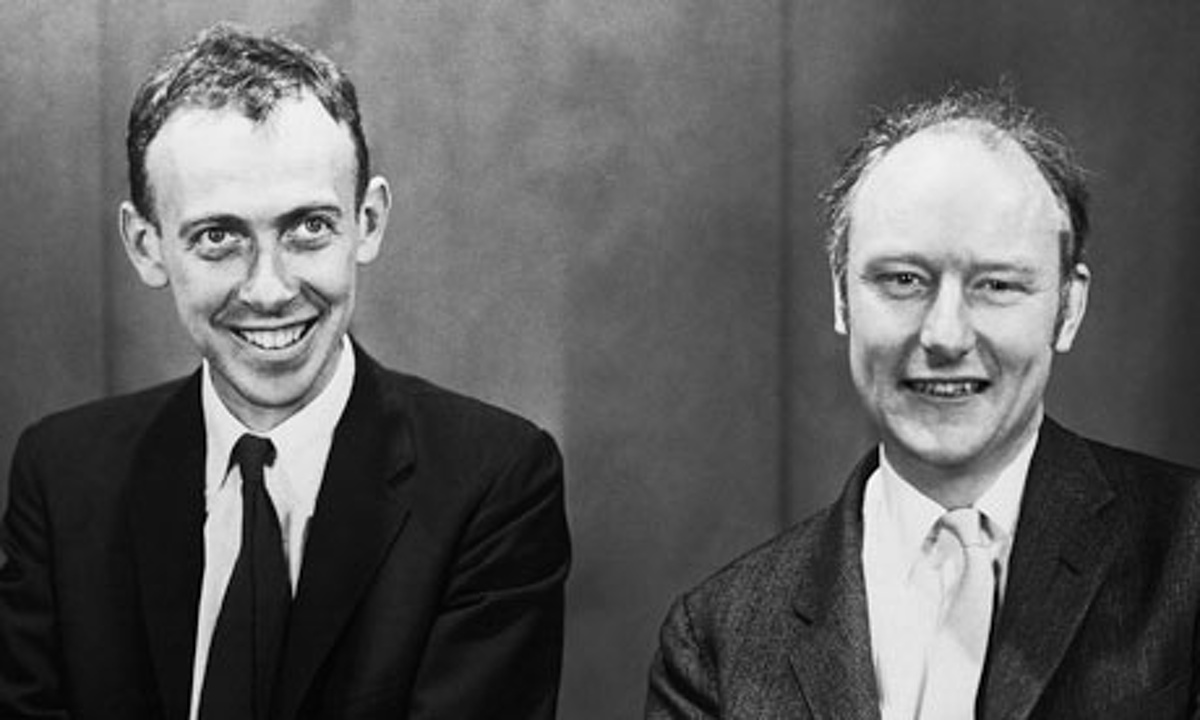
\includegraphics[scale=0.3]{JamesWatsonAndFrancisCrick.jpg}
     \caption{James Watson e Francis Crick}
     \label{fig:JamesWatsonAndFrancisCrick}
 \end{figure}
\vspace{1cm}

\indent \textbf{desenvolviento de métodos de SEQUENCIAMENTO de proteínas} \\

\indent Conforme o número de sequências de proteínas cresciam, aumentava também a necessidade de criar-se um banco de dados para indexá-las. A físico-química norte-americana Margaret Dayhoff, com colaboração de alguns membros do \textit{National Biomedical Research Foundation} em Washington, foi a primeira a contruir um banco de dados com este propósito em um tipo de atlas de proteínas na década de 60. Somente em 1984 esta coleção foi intitulada de \textit{Protein Information Resource} \cite{mount01}. Os dados eram organizados de acordo com o grau de similaridade das sequências, onde o agrupamento das mesmas era dado em forma de árvore filogenética representando famílias e superfamílias de proteínas. Caso a semelhança seja alta, é provável que tenham as mesmas funções bioquímicas e estrutura tridimensional. A partir da árvore gerada, foi possívei calcular as mutações que ocorreram nos aminoácidos durante a evolução genética e, então, produzir uma tabela utilizada até hoje, chamada PAM (\textit{percent acept mutation}), que apresenta tais dados. Outro banco de dados de grande porte e bastante utilizado nos dias de hoje é o GenBank, estabelecido em 1982 por Walter Goad e demais colaboradores e, agora, com o patrocínio do \textit{National Center for Biotechnology Information}. Os dois bancos são públicos e continuam crescendo exponencialmente \cite{mount01}.

\indent problemas ôminicos

\indent web search database david lipman




%  -------------------------------------------------------------
%  -------------------------------------------------------------

\indent A linha do tempo abaixo tem o objetivo de auxiliar na localização temporal da história da biologia molecular e da bioinformática ao passo que apresentam os maiores marcos dos principais pesquisadores da área. \\

%  -------------------------------------------- 
%  -------------------------------------------- LINHA DO TEMPO
%  -------------------------------------------- 

\begin{timeline}{1859}{1984}{2cm}{1cm}{13cm}{18cm}
\entry{1859}{Darwin publica livro A Origem das Espécies}
\entry{1865}{\textbf{Mendel apresenta pela primeira vez seu trabalho com ervilhas}}
\entry{1869}{Miescher identificou uma substância rica em fosfore na célula e a chamou de nucleína}
\entry{1871}{\textbf{Miescher publicou seu paper sobre a nucleína}}
\entry{1878}{Kossel obtém 5 bases nucléicas ao isolar parte não proteica da nucleína}
%\entry{1879}{Utilizando anilina, Flemming identifica a cromatina}
\entry{1882}{\textbf{Na divisão celular, Flemming identifica a formação dos cromossomos e chama o processo de mitose}}
\entry{1889}{Publicação do livro Intracellular Pangenesis, de Hugo de Vries}
\entry{1900}{\textbf{Vries publicou o artigo \textit{The Mutation Theory}}}
\entry{1909}{Johannsen introduziu a palavra gene ao vocabulário como característica específica de um organismo}
\entry{1913}{\textbf{Principal organismo utilizado para experiências genéticas é a \textit{Drosophila melanogaster}, utilizada por Thomas Morgan}}
\entry{1919}{Levene detectou três elementos que formam nucleotideos: um radical fosfato (HPO$_{4}$), uma pentose e uma base nitrogenada}
\entry{1933}{\textbf{Morgan recebe Prêmio Nobel de Fisiologia ou Medicina por provar a Teoria Cromossômica da Hereditariedade}}
\entry{1944}{Avery, McCarty e MacLeod provam que o DNA é o material hereditário}
\entry{1953}{\textbf{James Watson e Francis Crick descrevem a estrutura do DNA: a dupla hélice}}
\entry{1982}{Primeira versão do GenBank, na liderança de Walter Goad}
\entry{1984}{\textbf{Estabelecido o banco de dados Protein Information Resource, pela liderança de Magaret Dayhoff}}
\end{timeline}


% ADICIONAR DADOS: http://www.ncbi.nlm.nih.gov/pmc/articles/PMC2898077/figure/F2/

%  -------------------------------------------- 
%  -------------------------------------------- LINHA DO TEMPO
%  -------------------------------------------- 

\section{Problema e Hipótese}

\indent 
Contruir uma visualização interativa de redes metabólicas aramazenadas em banco de dados de grafos que permita ao pesquisador explorar os aspectos biológicos do organismo estudado.



\section{Justificativa}

\indent 
% Falar da quantidade de dados que e muito grande para ser examinada e o quanto um sistema com busca e uma visualizacao interativa
% pode auxiliar o pesquisador.

Atualmente, a quantidade de dados <<<<>>>> estudados pelos pesquisadores é extensa e complexa. Uma maneira de amenizar o esforço feito para analisá-los e compreendê-los é oferecer uma ferramenta que aproxime o usuário (pesquisador) e os dados em forma de grafo(redes metabólicas). Esta ferramenta deverá permitir que o usuário visualize e interaja com os dados dinamicamente, além de disponibilizar mecanismos de busca em grafos, úteis para sua pesquisa.


\section{Objetivo}

\indent 
Constrir um sistema que acesse redes metabólicas armazenadas em bancos de dados em grafo e gere uma visualização interativa
\begin{itemize}
 \item Implementar uma busca das vias metabólicas de interesse a apartir de parâmetros informados pelo pesquisador no sistema
 \item Recuperar a informação desejada e exibí-la para o pesquisador de forma ergonômica
 \item Implementar algoritmos de busca em grafos para recuperar a informação solicitada e/ou sugerir informação relevante
\end{itemize}

\section{Descrição dos Capítulos}

\indent No Capítulo 1 fez-se uma breve introdução à história da biologia molecular e da bioinformática. No Capítulo 2 são estabelecidas as principais definições utilizadas neste trabalho mais profundamente, tais como ácidos nucléidos, biomoléculas gerais que originam o DNA e o RNA; a proteína, macromolécula extensa, formada por um processo complexo chamado síntese de proteína; código genético, listagem do arranjo de bases nitrogenadas que formam aminoácidos, que por sua vez compõem a proteína; Neste capítulo também são descritos os processos de sequenciamento de proteínas, na subseção de bioinformática e os desafios enfrentados nessa área.

\indent O Capítulo 3 apresenta uma estrutura chamada Redes metabólicas, estrutura de dados extremamente complexas que existem para auxiliar o pesquisador biólogo a entender reações intracelulares, bem como determinar propriedades fisiológicas e bioquímicas das células. A construção destas redes é possível pos existe sequenciamento do genoma do organismo estudado. O Capítulo 4 propõe um banco de dados não relacional (NoDB) em grafos como maneira de armazenar estas redes metabólicas. Nele é descrito todo o conceito de NoDB, e é apresentado aquele utilizado neste trabalho: banco de dados OrientDB.

\indent No Capítulo 5 são exibidos os resultados da implementação do programa e no Capítulo 6, as conclusões tiradas a parir da análise dos dados. O Capítulo 7 expõe os problemas enfrentados, bem como sugestões de melhorias e trabalhos futuros. Por fim, o Capítulo 8 apresenta uma tabela do cronograma da execução deste trabalho.
